\begin{frame}{One-Sample Means}
    We can approach hypothesis testing for $\bar{x}$ in mostly the same way that we approached $\hat{p}$. However,
    \begin{itemize}
        \item We will often run into situations where $\bar{x}$ is not approximately normal.
        \item We will develop a framework for dealing with these situations.
    \end{itemize}
\end{frame}

\begin{frame}{The Central Limit Theorem for $\bar{x}$}
    When we collect a sufficiently large sample of $n$ independent observations from a population with mean $\mu$ and standard deviation $\sigma$, the sampling distribution of $\bar{x}$ will be nearly normal with mean
    \[
        \mu 
    \]
    and standard error
    \[
        \frac{\sigma}{\sqrt{n}}
    \]
\end{frame}

\begin{frame}{Conditions for Normality}
    For the Central Limit Theorem to hold, we require
    \begin{itemize}
        \item Independence
        \item Normality
    \end{itemize}
\end{frame}

\begin{frame}{Conditions for Normality: Independence}
    As before, for independence we typically check for 
    \begin{itemize}
        \item a simple random sample.
        \item a random process.
    \end{itemize}
\end{frame}

\begin{frame}{Conditions for Normality: Normality?}
    For $\bar{x}$ to be normally distributed,
    \begin{itemize}
        \item We require that the observations $x$ used to calculate $\bar{x}$ be from a normally distributed population.
        \item When this doesn't hold, we require a large sample size.
    \end{itemize}
\end{frame}

\begin{frame}{Large Sample Size}
    So what is a "large sample size"? 
    
    \vspace{12pt}$\boldsymbol{n < 30}$: A sample size $n$ less than 30 is considered a small sample. In this case, we will need the data to come from a nearly normal distribution.
    
    \vspace{12pt}$\boldsymbol{n \ge 30}$: A sample side $n$ of at least 30 is considered a large sample. Then we can assume that $\bar{x}$ is nearly normal.
    
    \vspace{12pt}In both cases, we need to be wary of outliers as these can cause problems with our results.
\end{frame}

\begin{frame}{Normal or Not?}
    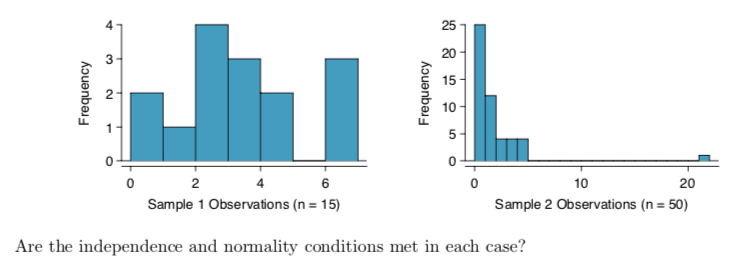
\includegraphics[scale=0.45]{images/normalorno.png}
\end{frame}

\begin{frame}{Normal or Not?}
    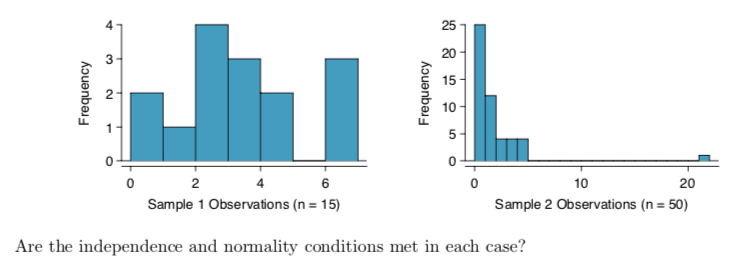
\includegraphics[scale=0.4]{images/normalorno.png}
    
    For the first plot, $n=15$ and there are no clear outliers. For the mean to be normally distributed, we would have to justify that these are draws from a normal distribution. 
\end{frame}

\begin{frame}{Normal or Not?}
    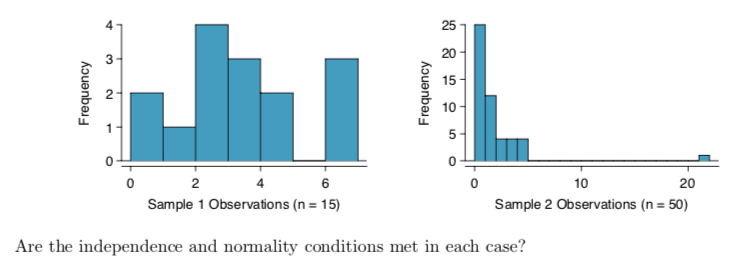
\includegraphics[scale=0.4]{images/normalorno.png}
    
    For the second plot, $n=50$ but there is an extreme outlier at about 22. This outlier will prevent us from confidently using a normal distribution. 
\end{frame}

\begin{frame}{One-Sample Means}
    We will start with the situation wherein we know that $X\sim N(\mu, \sigma)$ and the value of $\sigma$ is known.
\end{frame}

\begin{frame}{Confidence Interval for $\mu$}
    This $(1-\alpha)100\%$ confidence interval for $\mu$ is
    \[
       \bar{x} \pm z_{\alpha/2}\times\frac{\sigma}{\sqrt{n}} 
    \]
    where $\sigma/\sqrt{n}$ is the SE and $z_{\alpha/2}$ is again the critical value.
\end{frame}

\begin{frame}{Example}
    The following $n=5$ observations are from a $N(\mu, 2)$ distribution. Find a 90\% confidence interval for $\mu$.
    \[
        1.1, \quad 0.5, \quad 2, \quad 1.9, \quad 2.7
    \]
\end{frame}

\begin{frame}{Example}
    So we can be 90\% confident that the true mean $\mu$ is in the interval (0.1687, 3.1113). 
\end{frame}

\begin{frame}{Example}
    Recall that when we say "90\% confident", we mean:
    \begin{itemize}
        \item If we draw repeated samples of size 5 from this distribution, then 90\% of the time the corresponding intervals will contain the true value of $\mu$.
    \end{itemize}
\end{frame}

\begin{frame}{Confidence Interval for $\mu$}
    \begin{itemize}
        \item In practice, we typically do not know the population standard deviation $\sigma$.
        \item Instead, we have to estimate this quantity.
        \item We will use the sample statistic $s$ to estimate $\sigma$.
        \item This strategy works quite well when $n \ge 30$
    \end{itemize}
\end{frame}

\begin{frame}{Confidence Interval for $\mu$}
    This works quite well because we expect large samples to give us precise estimates such that
    \[
        SE = \frac{\sigma}{\sqrt{n}} \approx \frac{s}{\sqrt{n}}.
    \]
\end{frame}

\begin{frame}{Confidence Interval for $\mu$}
    When $n \ge 30$ and $\sigma$ is unknown, a $(1-\alpha)100\%$ confidence interval for $\mu$ is
    \[
        \bar{x} \pm z_{\alpha/2}\frac{s}{\sqrt{n}}
    \]
    where we've plugged in $s$ for $\sigma$.
\end{frame}

\begin{frame}{Example}
    The average heart rate of a random sample of 60 students is found to be 74 with a standard deviation of 11. Find a 95\% confidence interval for the true mean heart rate of the students. 
\end{frame}

\begin{frame}{Sample Size Calculation}
    Sample size calculation for means is essentially the same as for proportions!
    \[
        n \ge \left(\frac{z_{\alpha/2} \times sd}{MoE}\right)^2
    \]
\end{frame}

\begin{frame}{Example}
    A manufacturer claims with 95\% confidence that his product is accurate within 0.2 units with a standard deviation of 0.2626. What sample size would we need to demonstrate this claim?
\end{frame}

\begin{frame}{Hypothesis Testing for a Population Mean}
    We begin with the setting where $n\ge 30$. 
    \begin{itemize}
        \item As before, it is possible to use the confidence interval to complete a hypothesis test.
        \item However, we also want to be able to use our test statistic and p-value approaches.
    \end{itemize}
\end{frame}

\begin{frame}{Hypothesis Testing for a Population Mean}
    For $n \ge 30$, the test statistic is
    \[
        ts = z = \frac{\bar{x} - \mu_0}{s / \sqrt{n}}
    \]
    where again $s/\sqrt{n} \approx \sigma/\sqrt{n}$ because we are using a large sample.
\end{frame}

\begin{frame}{Hypothesis Testing for a Population Mean}
    There are five steps to carrying out these hypothesis tests:
    \begin{enumerate}
        \item Write out the null and alternative hypotheses.
        \item Calculate the test statistic.
        \item Use the significance level to find the critical value
            \begin{center}
                OR
            \end{center}
            use the test statistic to find the p-value.
        \item Compare the critical value to the test statistic
            \begin{center}
                OR
            \end{center}
            compare the p-value to $\alpha$.
        \item Conclusion.
    \end{enumerate}
\end{frame}

\begin{frame}{Example}
    In its native habitat, the average density of giant hogweed is 5 plants per $m^2$. In an invaded area, a sample of 50 plants produced an average of 11.17 plants per $m^2$ with a standard deviation of 8.9. Does the invaded area have a different average density than the native area? Test at the 5\% level of significance. 
\end{frame}

\begin{frame}{Hypothesis Testing for a Population Mean}
    We now move to the situation where $n < 30$. 
    
    \vspace{12pt}If $n < 30$ but we are dealing with a normal distribution and $\sigma$ is known,
    \[
        ts = z = \frac{\bar{x} - \mu_0}{\sigma / \sqrt{n}}
    \]
    but we know that this will rarely (if ever) occur in practice!
\end{frame}

\begin{frame}{Introducing the $t$-Distribution} 
    \begin{itemize}
        \item With a small sample size, plugging in $s$ for $\sigma$ can result in some problems.
        \item Therefore less precise samples will require us to make some changes.
        \item This brings us to the $t$-distribution.
    \end{itemize}
\end{frame}

\begin{frame}{Introducing the $t$-Distribution}
    The \textbf{$\boldsymbol{t}$-distribution} is a symmetric, bell-shaped curve like the normal distribution. 
    \begin{center}
        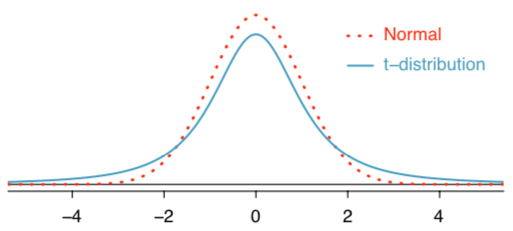
\includegraphics[scale=0.5]{images/tvsnrml.png}
    \end{center}
    
    However, the $t$-distribution has more area in the tails.
\end{frame}

\begin{frame}{Introducing the $t$-Distribution}
    \begin{center}
        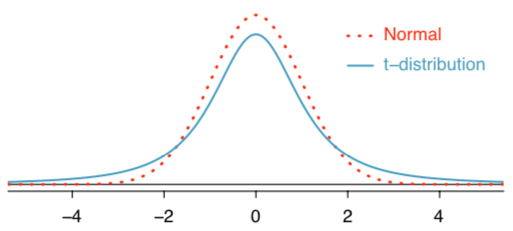
\includegraphics[scale=0.5]{images/tvsnrml.png}
    \end{center}
    
    These thicker tails turn out to be exactly the correction we need in order to use $s$ in place of $\sigma$ when calculating standard error!
\end{frame}

\begin{frame}{The $t$-Distribution}
    The $t$-distribution:
    \begin{itemize}
        \item Is always centered at zero.
        \item Has one parameter: degrees of freedom ($df$).
        \item For our purposes,
        \[
            df = n-1
        \]
        where $n$ is our sample size.
    \end{itemize}
\end{frame}

\begin{frame}{The $t$-Distribution}
    \begin{itemize}
        \item For the $t$-distribution, the parameter $df$ controls how fat the tails are.
        \item Higher values of $df$ result in thinner tails.
        \begin{itemize}
            \item That is, higher $df$ results in a $t$-distribution that looks more like a normal distribution.
            \item I.e., bigger sample sizes make the $t$-distribution look more normal.
        \end{itemize}
        \item When $n \ge 30$, the $t$-distribution will be essentially equivalent to the normal distribution.
    \end{itemize}
\end{frame}

\begin{frame}{Confidence Intervals for A Single Population Mean}
    When $n < 30$ and $\sigma$ is unknown, we use the $t$-distribution for our confidence intervals. A $(1-\alpha)100\%$ confidence interval for $\mu$ is
    \[
        \bar{x} \pm t_{\alpha/2, df} \times \frac{s}{\sqrt{n}}
    \]
\end{frame}

\begin{frame}{Critical Values for the $t$-Distribution}
    Let's take a minute to look at the table of $t$-distribution critical values that will be provided for your final exam. 
\end{frame}

\begin{frame}{Test Statistics}
    The test statistic for the setting where $n < 30$ and $\sigma$ is unknown is
    \[
        ts = t = \frac{\bar{x}-\mu_0}{s/\sqrt{n}}
    \]
    (two-sided hypotheses)
\end{frame}

\begin{frame}{P-Values}
    The p-value for the two-sided hypotheses is then
    \[
        2\times P(t_{df} < -|ts|)
    \]
\end{frame}

\begin{frame}{Example}
    The following data is on red blood cell counts (in $10^6$ cells per microliter) for 9 people:
    \[
        5.4, \quad 5.3, \quad 5.3, \quad 5.2, \quad 5.4, \quad 4.9, \quad 5.0, \quad 5.2, \quad 5.4
    \]
    Test at the 5\% level of significance if the average cell count is 5.
\end{frame}